\chapter{Anhang }
\label{cha:Anhang}

\section{GDBMS-Implementierungen}
\label{anh:vendor_list}

\renewcommand{\arraystretch}{1.25}
\begin{table}[h]
	\centering
	\begin{footnotesize}
   	\begin{tabular}{|m{2.5cm}|m{3.5cm}|>{\arraybackslash}m{9.25cm}|}
	\hline	
	\textbf{GDBMS} & \textbf{Hersteller} & \textbf{Website} \\
	\hline
   	Affinity 		& GoPivotal 			& \url{http://affinityng.cfapps.io/} \\
   	ArangoDB 		& triAGENS 				& \url{http://www.arangodb.org/} \\
   	Bitsy 			& Privatperson 			& \url{https://bitbucket.org/lambdazen/bitsy/} \\
   	DEX 			& Sparsity Technologies & \url{http://www.sparsity-technologies.com/dex} \\
   	Filament 		& Privatperson 			& \url{http://sourceforge.net/projects/filament/} \\
   	FlockDB 		& Twitter				& \url{https://github.com/twitter/flockdb} \\
   	GraphBase 		& FactNexus 			& \url{http://graphbase.net/} \\
   	GraphPack 		& Privatperson 			& \url{https://code.google.com/p/graphpack/} \\
   	G-Store 		& Forschungsprototyp	& \url{http://g-store.sourceforge.net/} \\
   	Horton 			& Microsoft 			& \url{http://research.microsoft.com/en-us/projects/ldg/} \\
   	HyperGraphDB 	& Kobrix Software		& \url{http://www.hypergraphdb.org/index} \\
   	InfiniteGraph 	& Objectivity			& \url{http://www.objectivity.com/infinitegraph} \\
   	Fallen-8 		& Privatperson 			& \url{http://www.fallen-8.com/} \\
   	Neo4j 			& Neo Technology 		& \url{http://www.neo4j.org/} \\
   	OQGRAPH 		& Open Query 			& \url{http://openquery.com/node/23} \\
   	OrientDB 		& Orient Technologies 	& \url{http://www.orientdb.org/} \\
   	RedisGraph 		& Privatperson 			& \url{https://github.com/tblobaum/redis-graph} \\
   	SGDB3 			& Forschungsprototyp 	& \url{http://ups.savba.sk/~marek/sgdb.html} \\
   	Titan 			& Aurelius 				& \url{http://thinkaurelius.github.io/titan/} \\
   	Trinity 		& Microsoft 			& \url{http://research.microsoft.com/en-us/projects/trinity/} \\
   	VertexDB 		& Privatperson 			& \url{https://github.com/stevedekorte/vertexdb} \\
   	\hline
   	\end{tabular} 
	\end{footnotesize}
	\setlength{\belowcaptionskip}{0.25cm}	
	\caption[GDBMS-Hersteller]{Liste der Webseiten untersuchter GDBMS.}
	\label{tab:anh_urls}
\end{table}
\renewcommand{\arraystretch}{1}

\section{Quellcodebeispiele}

Abbildung \ref{fig:example} zeigt die Instanz eines Property-Graph, welche in den nachfolgenden Beispielen verwendet wird, das verwendete Schema entspricht dem Schema im Benchmark.

\begin{figure}[h] 
	\centering
		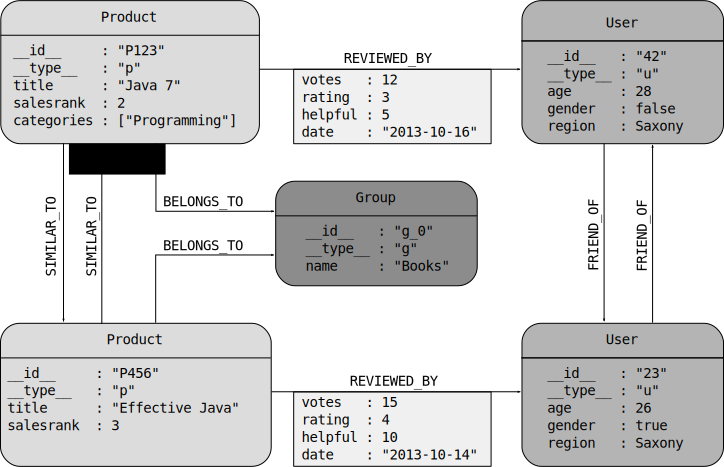
\includegraphics[scale=.75]{example.pdf}
	\caption[Anhang: Beispielgraph]{Datengrundlage f�r Quellcodebeispiele.}
	\label{fig:example}
\end{figure}

\subsection*{Neo4j}
\label{anh:neo4j_api}

\lstset{language=Java, basicstyle=\ttfamily\footnotesize, caption={CRUD-Operationen Neo4j Core API}, label=list:sim_products_gremlin}
\begin{lstlisting}
try (Transaction tx = graphDB.beginTx()) {
	Label productLabel = new Label() {@Override public String name() { 
		return "Product"; }};
	Label userLabel = new Label() {@Override public String name() {
	    return "User";
	}};
	// create node with label "Product"
	Node p123 = graphDB.createNode(productLabel);
	p123.setProperty("__id__", "P123");
	p123.setProperty("__type__", "p");
	p123.setProperty("title", "Effective Java");
	p123.setProperty("salesrank", 2);
	p123.setProperty("categories", new String[] { "Programming" });
	// create node with label "User"
	Node u42 = graphDB.createNode(userLabel);
	u42.setProperty("__id__", "42");
	u42.setProperty("__type__", "u");
	u42.setProperty("age", 28);
	u42.setProperty("gender", false);
	u42.setProperty("region", "Saxony");
	// create edge from product to user
	Relationship review1 = p123.createRelationshipTo(u42, 
		RelTypes.REVIEWED_BY);
	review1.setProperty("votes", 12);
	review1.setProperty("rating", 3);
	review1.setProperty("helpful", 5);
	review1.setProperty("date", "2013-10-06");
}
\end{lstlisting}

\subsection*{HypergraphDB}

\subsection*{OrientDB}

\subsection*{Titan}

\section{Benchmark}



\subsection{Extraktion}
\label{anh:extraction}

\subsection{Operationen}
\label{anh:queries}

% random read
\subsubsection*{\texttt{random\_read}}

\lstset{language=Java, caption={Operation \texttt{random\_read} in Cypher}, label=list:random_read_cypher}
\begin{lstlisting}
START a=node(42) RETURN *;
\end{lstlisting}

\lstset{language=Java, caption={Operation \texttt{random\_read} in Gremlin}, label=list:random_read_gremlin}
\begin{lstlisting}
g.v(42).map();
\end{lstlisting}

% sim products
\subsubsection*{\texttt{sim\_products}}

\lstset{language=Java, caption={Operation \texttt{sim\_products} in Cypher}, label=list:sim_products_cypher}
\begin{lstlisting}
START n=node(42) 
MATCH n-[:SIMILAR_TO*..2]-s 
RETURN DISTINCT s.title AS title;
\end{lstlisting}

\lstset{language=Java, caption={Operation \texttt{sim\_products} in Gremlin}, label=list:sim_products_gremlin}
\begin{lstlisting}
g.v(42).both('SIMILAR_TO').loop(1){it.loops <= 2}.dedup().title;
\end{lstlisting}

% foaf reviews
\subsubsection*{\texttt{foaf\_reviews}}

\lstset{language=Java, caption={Operation \texttt{foaf\_reviews} in Cypher}, label=list:foaf_reviews_cypher}
\begin{lstlisting}
START n=node(42)
MATCH n-[:FRIEND_OF*1..2]-()<-[r:REVIEWED_BY]-p
RETURN p.title AS title, avg(r.rating) AS weight
ORDER BY weight DESC;
\end{lstlisting}

\lstset{language=Java, caption={Operation \texttt{foaf\_reviews} in Gremlin}, label=list:foaf_reviews_gremlin}
\begin{lstlisting}
g.v(42).both('FRIEND_OF').both('FRIEND_OF').inE('REVIEWED_BY')
	.groupBy{it.outV.next().title}{it.rating}{it.sum() * 1.0 / it.size()}
	.cap.orderMap(T.decr);
\end{lstlisting}

% path all
\subsubsection*{\texttt{path\_all}}

\lstset{language=Java, caption={Operation \texttt{path\_all} in Cypher}, label=list:path_all_cypher}
\begin{lstlisting}
START a=node(42), b=node(23) 
MATCH p=a-[:FRIEND_OF|SIMILAR_TO|REVIEWED_BY*..4]-b 
RETURN length(p) AS length, count(p) AS cnt;
\end{lstlisting}

\lstset{language=Java, caption={Operation \texttt{path\_all} in Gremlin}, label=list:path_all_gremlin}
\begin{lstlisting}
a = g.v(42);
b = g.v(23);
visited=[a];
a.both('FRIEND_OF','REVIEWED_BY','SIMILAR_TO')
	.loop(1){it.object != b && it.loops < 5}.retain([b])
	.path._().transform{it.size() - 1}.groupCount().cap();
\end{lstlisting}

% path shortest
\subsubsection*{\texttt{path\_shortest}}

\lstset{language=Java, caption={Operation \texttt{path\_shortest} in Cypher}, label=list:path_shortest_cypher}
\begin{lstlisting}
START a=node(42), b=node(23)
MATCH p=shortestPath(a-[:FRIEND_OF|:REVIEWED_BY|:SIMILAR_TO*..5]-b)
RETURN EXTRACT(n in NODES(p): n.__id__) AS path;
\end{lstlisting}

\lstset{language=Java, caption={Operation \texttt{path\_shortest} in Gremlin}, label=list:path_shortest_gremlin}
\begin{lstlisting}
a = g.v(42);
b = g.v(23);
visited=[a];
a.both('FRIEND_OF', 'REVIEWED_BY', 'SIMILAR_TO')
	.except(visited).store(visited)
	.loop(3){it.object != b && it.loops < 6}.retain([b])
	.path{it.__id__};
\end{lstlisting}

% top regions
\subsubsection*{\texttt{top\_regions}}

\lstset{language=Java, caption={Operation \texttt{top\_region} in Cypher}, label=list:top_region_cypher}
\begin{lstlisting}
START g=node:nodes('__id__':'g_0')
MATCH g<-[:BELONGS_TO]-p-[r:REVIEWED_BY]->u
WHERE p.salesrank < 500000
RETURN u.region AS region, count(u) AS cnt
ORDER BY cnt DESC
LIMIT 10;
\end{lstlisting}

\lstset{language=Java, caption={Operation \texttt{top\_region} in Gremlin}, label=list:top_region_gremlin}
\begin{lstlisting}
group = g.V('__id__', 'g_0').next();
group.in('BELONGS_TO').filter{it.salesrank < 500000}
	.out('REVIEWED_BY').groupCount{it.region}.cap()
	.orderMap(T.decr)[0..9];
\end{lstlisting}

% sim pattern
\subsubsection*{\texttt{sim\_pattern}}

\lstset{language=Java, caption={Operation \texttt{sim\_pattern} in Cypher}, label=list:sim_pattern_cypher}
\begin{lstlisting}
START user=node(42)
MATCH user-[:FRIEND_OF]-friends1<-[:REVIEWED_BY]-products,
products-[:REVIEWED_BY]->friends2
WITH user, products, collect(distinct friends1.__id__) as f1, collect(distinct friends2.__id__) as f2
WITH user, products, filter(x in f1 : x in f2) as intersect
WITH user, products, count(products) as n, intersect, length(intersect) as intersect_cnt
WHERE intersect_cnt > 1 and n > 0
RETURN user.__id__ as user_id, n, products.__id__ as product_id, intersect as friends, intersect_cnt;
\end{lstlisting}

\lstset{language=Java, caption={Operation \texttt{sim\_pattern} in Gremlin}, label=list:sim_pattern_gremlin}
\begin{lstlisting}
u = g.v(42);
m = [:]; common_products = [] as Set;
u.both("FRIEND_OF").dedup().transform({ it.in("REVIEWED_BY").dedup() })
	.scatter().groupCount(m).filter({ m[it] >= 2 }).fill(common_products);
common_products._().as("product").transform({
	it.out("REVIEWED_BY").filter({
		it.in("REVIEWED_BY").retain(common_products)[0..<2].count() == 2
	}).as("friend").both("FRIEND_OF").retain([u]).back("friend").toSet()
}).as("friends").table().cap().next();
\end{lstlisting}



